%%%%%%%%%%%%%%%%%%%%%%%%%%%%%%%%%%%%%%%%%%%%%%%%%%%%%%%%%%%%
%%  This Beamer template was created by Cameron Bracken.
%%  Anyone can freely use or modify it for any purpose
%%  without attribution.
%%
%%  Last Modified: January 9, 2009
%%

\documentclass[xcolor=x11names,compress]{beamer}

%% General document %%%%%%%%%%%%%%%%%%%%%%%%%%%%%%%%%%
\usepackage{graphicx}
\usepackage{tikz}
\usepackage[english]{babel}
\usepackage[T1]{fontenc}
\usepackage[utf8]{inputenc}
\usepackage{hyperref}
\usepackage{listings}
\usepackage{textcomp}

\lstset{
	numbers=none,
	numberstyle=\tiny,
	basicstyle=\scriptsize,
	numbersep=5pt,
	showstringspaces=false
	}
%\usetikzlibrary{decorations.fractals}
%%%%%%%%%%%%%%%%%%%%%%%%%%%%%%%%%%%%%%%%%%%%%%%%%%%%%%


%% Beamer Layout %%%%%%%%%%%%%%%%%%%%%%%%%%%%%%%%%%
\useoutertheme[subsection=false,shadow]{miniframes}
\useinnertheme{default}
\usefonttheme{serif}
\usepackage{palatino}

\setbeamerfont{title like}{shape=\scshape}
\setbeamerfont{frametitle}{shape=\scshape}

\definecolor{CSPIGreen}{RGB}{119,188,31}
\definecolor{CSPIBlue}{RGB}{0,78,176}
\definecolor{CSPIBlack}{RGB}{61,56,52}

\setbeamercolor*{lower separation line head}{bg=CSPIGreen} 
\setbeamercolor*{normal text}{fg=black,bg=white}
\setbeamercolor*{alerted text}{fg=CSPIBlue} 
\setbeamercolor*{example text}{fg=black} 
\setbeamercolor*{structure}{fg=black} 
 
\setbeamercolor*{palette tertiary}{fg=black,bg=black!10}
\setbeamercolor*{palette quaternary}{fg=black,bg=black!10}

\renewcommand{\(}{\begin{columns}}
\renewcommand{\)}{\end{columns}}
\newcommand{\<}[1]{\begin{column}{#1}}
\renewcommand{\>}{\end{column}}

%%%%%%%%%%%%%%%%%%%%%%%%%%%%%%%%%%%%%%%%%%%%%%%%%%%%%%%
%%%%%%%%%%% YAML syntax highlighting %%%%%%%%%%%%%%%%%

% http://tex.stackexchange.com/questions/152829/how-can-i-highlight-yaml-code-in-a-pretty-way-with-listings

% here is a macro expanding to the name of the language
% (handy if you decide to change it further down the road)
\newcommand\YAMLcolonstyle{\color{red}\mdseries}
\newcommand\YAMLkeystyle{\color{black}\bfseries}
\newcommand\YAMLvaluestyle{\color{blue}\mdseries}

\makeatletter

\newcommand\language@yaml{yaml}

\expandafter\expandafter\expandafter\lstdefinelanguage
\expandafter{\language@yaml}
{
  keywords={true,false,null,y,n},
  keywordstyle=\color{darkgray}\bfseries,
  basicstyle=\YAMLkeystyle,                                 % assuming a key comes first
  sensitive=false,
  comment=[l]{\#},
  morecomment=[s]{/*}{*/},
  commentstyle=\color{purple}\ttfamily,
  stringstyle=\YAMLvaluestyle\ttfamily,
  moredelim=[l][\color{orange}]{\&},
  moredelim=[l][\color{magenta}]{*},
  moredelim=**[il][\YAMLcolonstyle{:}\YAMLvaluestyle]{:},   % switch to value style at :
  morestring=[b]',
  morestring=[b]",
  literate =    {---}{{\ProcessThreeDashes}}3
                {>}{{\textcolor{red}\textgreater}}1     
                {|}{{\textcolor{red}\textbar}}1 
                {\ -\ }{{\mdseries\ -\ }}3,
}

% switch to key style at EOL
\lst@AddToHook{EveryLine}{\ifx\lst@language\language@yaml\YAMLkeystyle\fi}
\makeatother

\newcommand\ProcessThreeDashes{\llap{\color{cyan}\mdseries-{-}-}}

%%%%%%%%%%% YAML syntax highlighting %%%%%%%%%%%%%%%%%
%%%%%%%%%%%%%%%%%%%%%%%%%%%%%%%%%%%%%%%%%%%%%%%%%%%%%%

%%%%%%%%%%%%%%%%%%%% VARIABLES %%%%%%%%%%%%%%%%%%%%%%%

\def \Author {Oleg Fiksel}
\def \AuthorEmail {\href{mailto:oleg.fiksel@cspi.com}{oleg.fiksel@cspi.com}}

%%%%%%%%%%%%%%%%%%%%%%%%%%%%%%%%%%%%%%%%%%%%%%%%%%%%%%

%%%%%%%%%%%%%%%%%%%%%%%%%%%%%%%%%%%%%%%%%%%%%%%%%%%%%%
\begin{document}
%%%%%%%%%%%%%%%%%%%%%%%%%%%%%%%%%%%%%%%%%%%%%%%%%%%%%%
%%%%%%%%%%%%%%%%%%%%%%%%%%%%%%%%%%%%%%%%%%%%%%%%%%%%%%

\begin{frame}
\title{Taskwarrior}
\subtitle{Todo-Liste für Geeks}
\author{
	\textbf{\Author}\\[1em]
	\begin{it}
	 Security Consultant @ CSPI GmbH\\[1em]
	 \begin{footnotesize}
		\AuthorEmail \hspace{0.5pt} \textbar \hspace{0.5pt} \href{mailto:oleg@fiksel.info}{oleg@fiksel.info}
	 \end{footnotesize}
	 \end{it}
}
\date{OpenRheinRuhr 2015}
\titlepage
\end{frame}

%%%%%%%%%%%%%%%%%%%%%%%%%%%%%%%%%%%%%%%%%%%%%%%%%%%%%%
%%%%%%%%%%%%%%%%%%%%%%%%%%%%%%%%%%%%%%%%%%%%%%%%%%%%%%
\begin{frame}{Agenda}
\tableofcontents
\end{frame}

%%%%%%%%%%%%%%%%%%%%%%%%%%%%%%%%%%%%%%%%%%%%%%%%%%%%%%
%%%%%%%%%%%%%%%%%%%%%%%%%%%%%%%%%%%%%%%%%%%%%%%%%%%%%%

\section{\scshape{About}}

\subsection*{Me}
\begin{frame}{About me}
	\begin{itemize}
		\item Security Consultant at CSPI (former MODCOMP)
		\item \textbf{Main topics}
			\begin{itemize}
				\item Automation
				\item Virtualisation
				\item Application Switching (load balancing)
				\item Perl Coding
			\end{itemize}
	\end{itemize}
\end{frame}

\subsection*{Company}

\begin{frame}{About MODCOMP}
	\begin{itemize}
		\item Founded in 1976 as MODCOMP Inc.\\ Since 1985 in Germany.
		\item Main scope: production of minicomputer for real-time environments.\\ Example: NASA Space Shuttle Program.
		\item Development of real-time operating system Real/IX.
		\item 1990 - 1992 Cray and Bull equip their HPCs with Real/IX.
		\item 1995 New scope: Security Consulting.
		\item 1996 Purchased by CSPI.
		\item Since 2015 re-branded as CSPI Germany.
	\end{itemize}
\end{frame}

\begin{frame}{About CSPI}
	\begin{itemize}
		\item 3 locations world wide: US, DE, UK.
		\item CSPI Germany (Köln) \texttildelow 90 employees.
		\begin{itemize}
			\item 9 solution centers covering every aspect of IT-Security.
			\item An opportunity to work on big infrastructures with cutting edge technology.
		\end{itemize}
	\end{itemize}
\end{frame}

\section{\scshape{Introduction}}

\subsection{Goals of this talk}

\begin{frame}{Goals of this talk}
\pause
	\begin{itemize}[<+-| alert@+>]
			\setlength\itemsep{2em}
			\item Clarify why task management is important
			\item Provide a short summary of main point from popular time management techniques
			\item Introduction to Taskwarrior
	\end{itemize}
\end{frame}

\section{\scshape{Tasks for human beings}}

\subsection{Problem}
\begin{frame}{Problem}
	\begin{itemize}[<+-| alert@+>]
			\item We are not robots (most of us)
			\item We need motivation to do our tasks
			\item Sometimes we work all day but don't have an impression we did something
	\end{itemize}
\end{frame}

\subsection{Purpose of a Task-Application}
\begin{frame}{Purpose of a Task-Application}
	\begin{itemize}[<+-| alert@+>]
			\item A task list application will not solve your todos
			\item It's just a tool to help organize and \textbf{get an overview}
			\item A task list is only usefull if you have an overview \textit{(priorities)}
			\item A task list should be easy to use
	\end{itemize}
\end{frame}

\subsection{GTD}

\begin{frame}{GTD}
 
\end{frame}

\begin{frame}{GTD}
\begin{center}
\textbf{GTD}
\pause
 ( \textbf{G}etting \textbf{T}hings \textbf{D}one )
\pause
\textit{ - is a time-management method, described in a book of the same title by productivity consultant David~Allen. \footnotemark[1]}
\end{center}
\footnotetext[1]{\href{https://en.wikipedia.org/wiki/Getting_Things_Done}{Wikipedia Quote}}
\end{frame}

\subsection{Some of GTD principles}

\begin{frame}{Some of GTD principles}
\pause
	\begin{itemize}[<+-| alert@+>]
		\item Task takes $\leq$ 5 minutes $\rightarrow$ do it
		\item Task takes $>$ 5 minutes $\rightarrow$ schedule/plan it
		\item Split big tasks into small ones
		\item Task/Idea $\rightarrow$ write down (and schedule for a review)
		\item Have Long-Term Tasks
		\begin{itemize}[<+-| alert@+>]
			\item \textit{Example: Proceeed with learning Perl each Sunday}
		\end{itemize}
		\item Nice-to-have tasks for free time
		\begin{itemize}
			\item \textit{Example: Do a PoC with Taskwarrior}
			\item \textit{Example: Read an article about GTD with Taskwarrior}
		\end{itemize}
		\item Do every morning a Task review and schedule your day
	\end{itemize}
\end{frame}

\subsection{In addition to GTD}
\begin{frame}{In addition to GTD}
\pause
	\begin{itemize}[<+-| alert@+>]
		\item Try to do the unpleasant tasks first in the morning
		\item Treat yourself with some pleasant tasks at the end of the day
		\item Put all needed informations in the a task (as you would deligate the task to someone) $\rightarrow$ keeps your head free
		\item Handle tasks with context
		\begin{itemize}
			\item \textit{Example: ``Buy milk'' task in a grocery store (not at home)}
		\end{itemize}
		\item Task switching takes additional time (could be a performance-killer for programmers)
		\begin{itemize}
			\item \textit{for extremists: \href{https://en.wikipedia.org/wiki/Pomodoro_Technique}{Pomodoro Technique}}
		\end{itemize}
	\end{itemize}
\end{frame}

\section{Taskwarrior}

\subsection{Why Taskwarrior?}
\begin{frame}{Why Taskwarrior?}
\pause
My motivation was to find:
\pause
	\begin{itemize}[<+-| alert@+>]
		\item Open Source
		\item Multi-Platform (Linux, Android, MacOS, BSD, ...)
		\item Secure (SSL, PKI)
		\item Self-Hosted
		\begin{itemize}
			\item Client-Server Model
			\item Privacy aware
			\begin{itemize}
				\item \textit{Example todo: move the money to Switzerland (Taxman)}
			\end{itemize}
		\end{itemize}
		\item lighweight \textit{(Redmine, Jira)}
		\item efficient to use \textit{(Redmine, Jira)}
		\item Mobile Client (Android)
		\begin{itemize}
			\item \textit{IMHO: task list isn't usefull if you don't have it with you all the time}
		\end{itemize}
	\end{itemize}
\end{frame}

\subsection{Architecture}
\begin{frame}[fragile]{Taskwarrior architecture}
	\begin{center}
		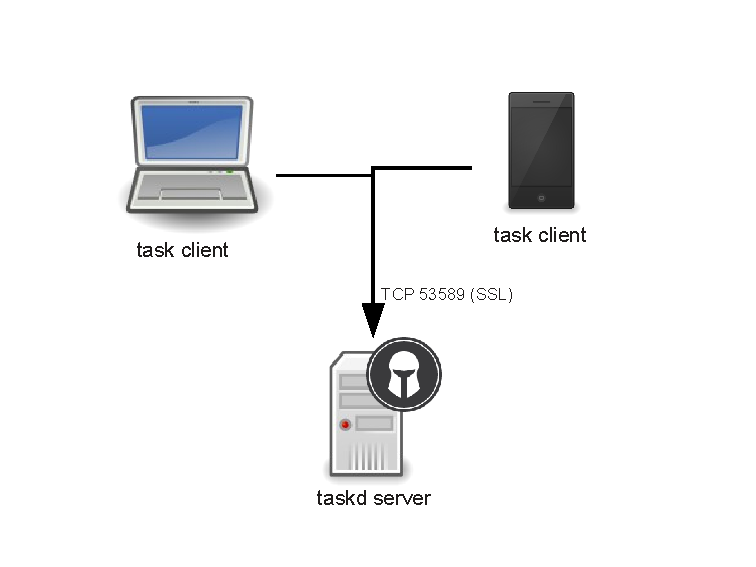
\includegraphics[height=7.5cm]{taskwarrior_architecture.pdf}
	\end{center}
\end{frame}

\section{Summary}
\subsection*{Summary}
\begin{frame}[fragile]{Summary}
\pause
	\begin{itemize}[<+-| alert@+>]
		\setlength\itemsep{2em}
		\item Marking tasks as done makes you happy and motivated to do other tasks
		\item Right task management makes handling your tasks easier and reduces stress
		\item Taskwarrior helps you accomplish this \\ $\rightarrow$ \textit{task add due:sunday try Taskwarrior}
		\item Doing tasks can be addictive. \\ Try to maintain a Tasks-Life balance. \\ $\rightarrow$ \textit{task add due:today recur:daily Watch out of the window and calm down from a stressed day}
	\end{itemize}
\end{frame}

\section{\scshape{Demo}}


\subsection*{Demo}
\begin{frame}[fragile]{}
	\begin{center}
		\huge{Demo}
	\end{center}
\end{frame}

\subsection*{Reporting: summary}
\begin{frame}[fragile]{Reporting: summary}
	\begin{center}
		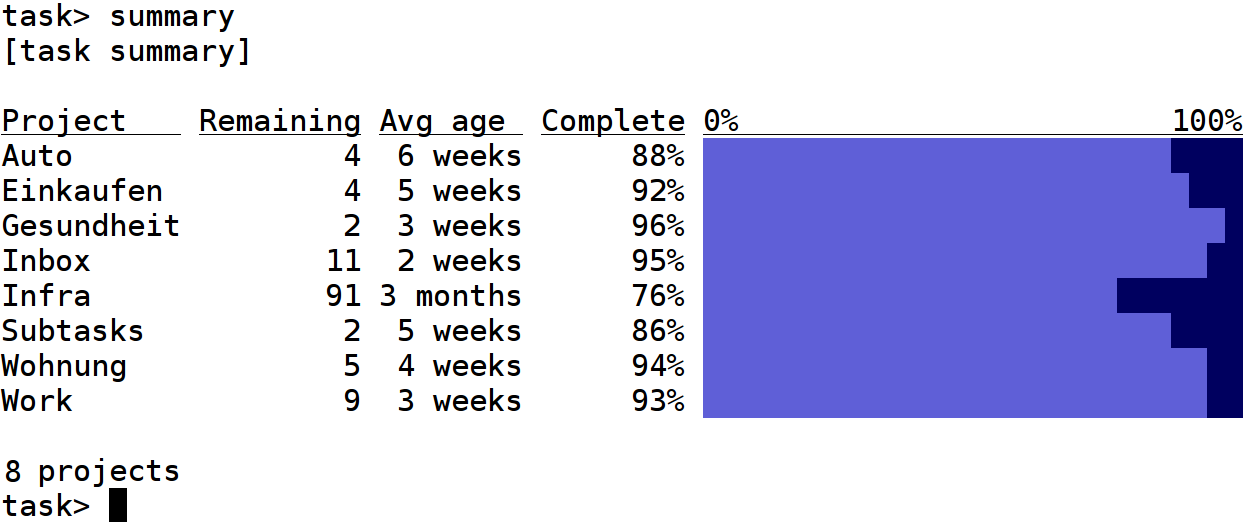
\includegraphics[width=10.5cm]{screenshots/summary.png}
	\end{center}
\end{frame}

\subsection*{Reporting: burndown}
\begin{frame}[fragile]{Reporting: burndown}
	\begin{center}
		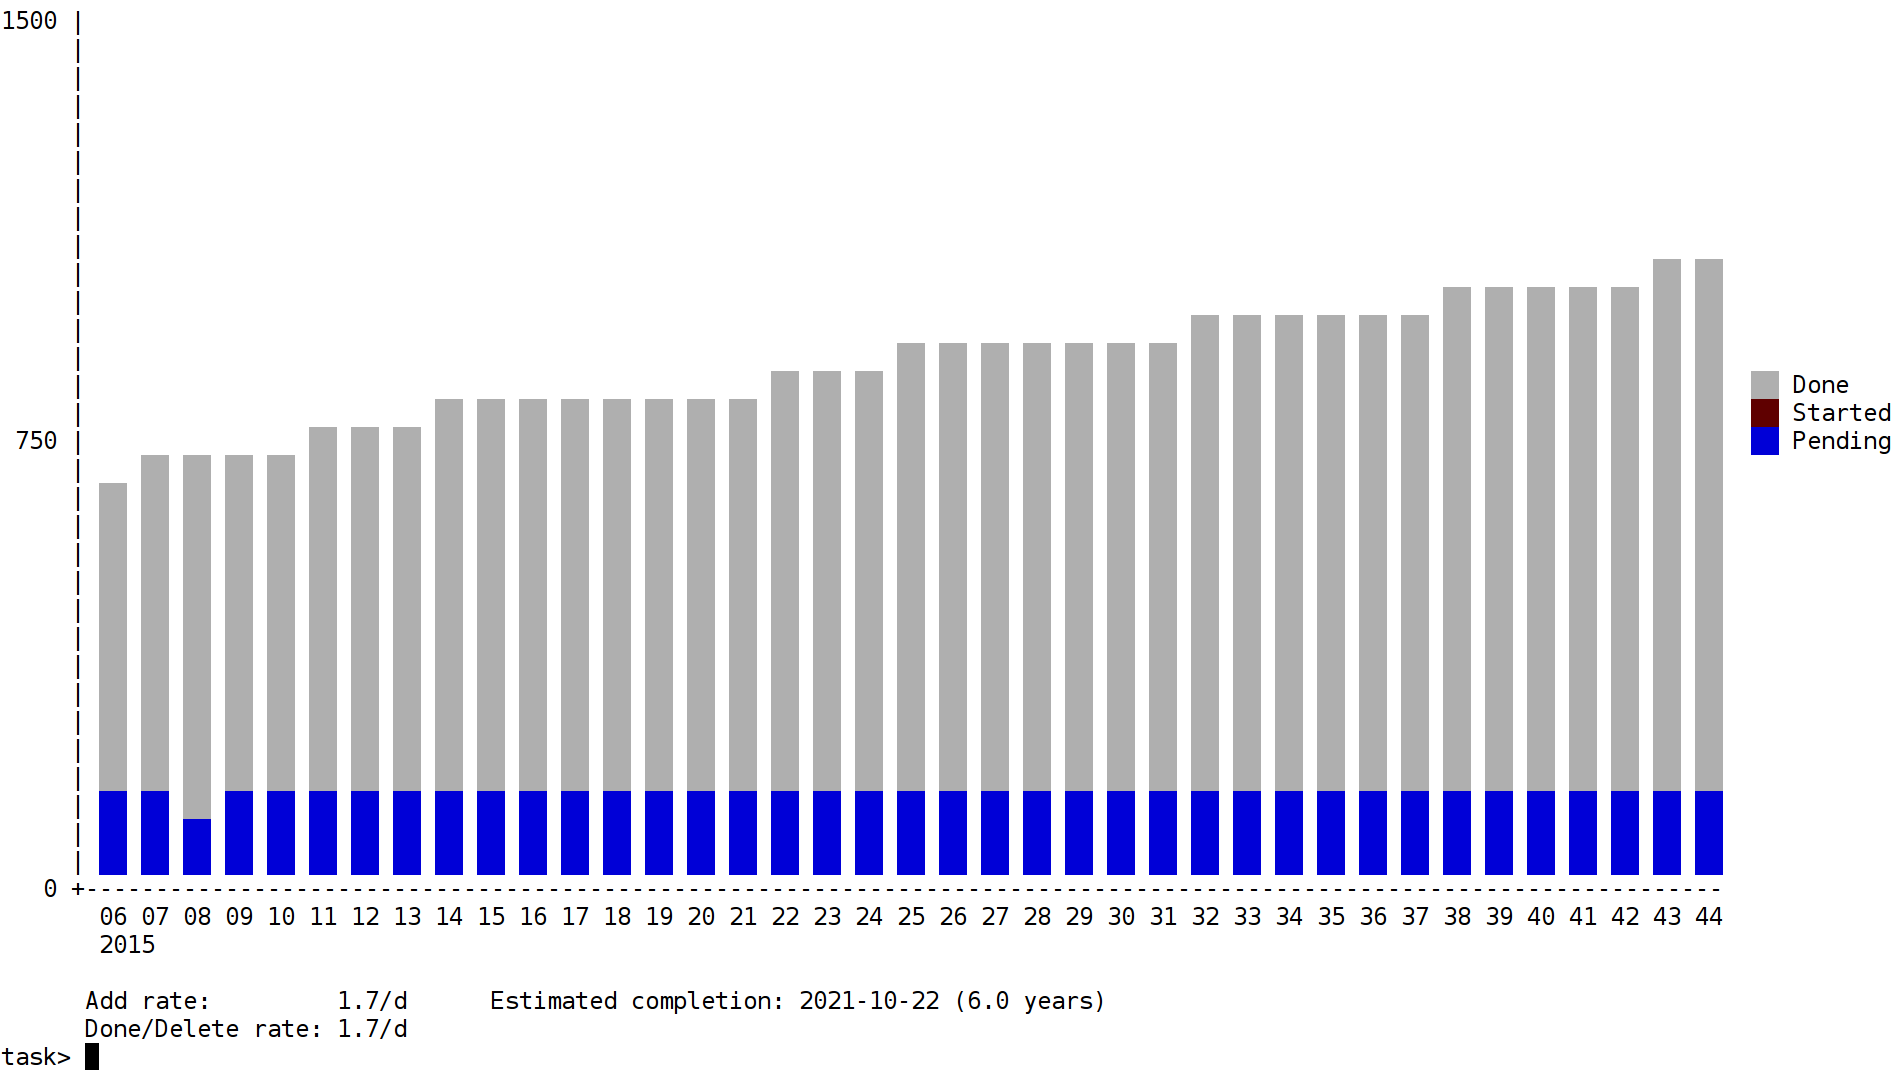
\includegraphics[width=10.5cm]{screenshots/burndown.png}
	\end{center}
\end{frame}

\subsection*{Reporting: ghistory}
\begin{frame}[fragile]{Reporting: ghistory}
	\begin{center}
		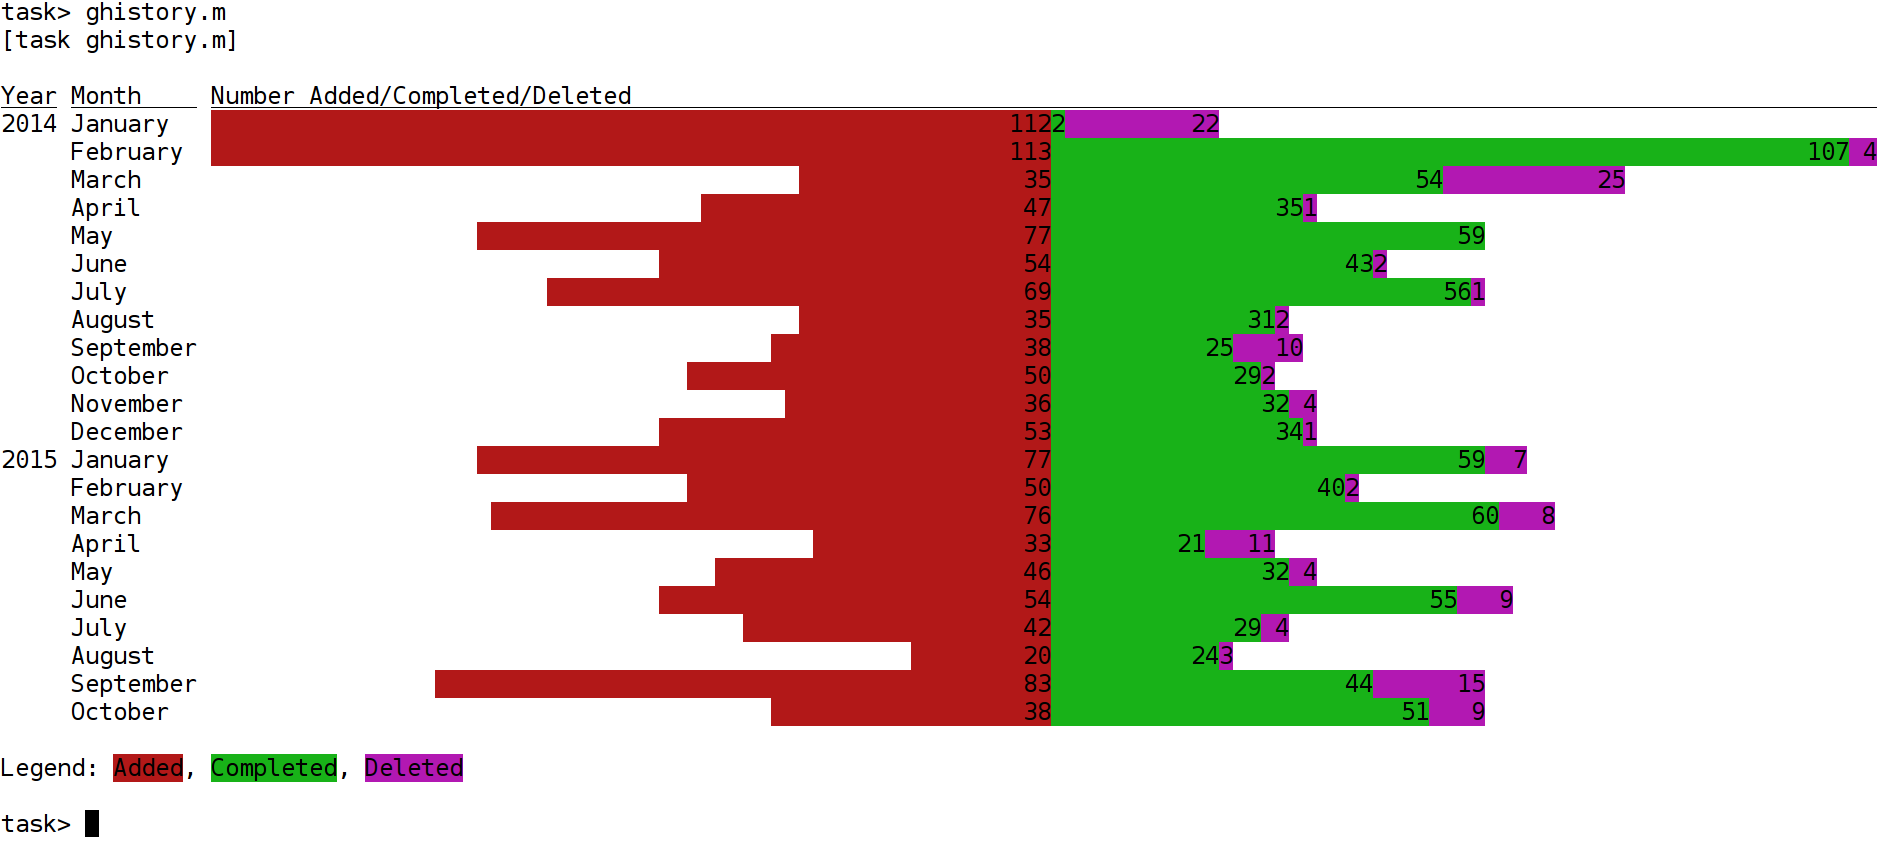
\includegraphics[width=10.5cm]{screenshots/ghistory.png}
	\end{center}
\end{frame}

\section{\scshape{End}}

\subsection{Q \& A}
\begin{frame}[fragile]{}
\begin{center}
	\huge{Q \& A}
\end{center}
\end{frame}

\subsection{Links}

\begin{frame}[fragile]{Links}
	\begin{itemize}
		\item MODCOMP/CSPI
		\begin{itemize}
			\item \href{http://www.cspi.com/de/uber/history}{MODCOMP History}
			\item \href{https://en.wikipedia.org/wiki/MODCOMP}{MODCOMP on Wikipedia}
		\end{itemize}
		\item Taskwarrior
		\begin{itemize}
			\item \href{http://taskwarrior.org/docs/}{Taskwarrior Docs}
			\item \href{http://mirakel.azapps.de/}{Taskwarrior Android Client (Mirakel)}
		\end{itemize}
		\item GTD
		\begin{itemize}
			\item \href{https://en.wikipedia.org/wiki/Getting_Things_Done}{GTD on Wikipedia}
			\item \href{https://en.wikipedia.org/wiki/Pomodoro_Technique}{Pomodoro Technique on Wikipedia}
		\end{itemize}
	\end{itemize}
\end{frame}

\begin{frame}[fragile]{Links}
	Go deep: Dirk Deimeke's talks \vspace{3pt}
	\begin{itemize}
		\item \href{https://speakerdeck.com/ddeimeke/taskwarrior-whats-next-1}{Taskwarrior: What's next 1}
		\item \href{https://speakerdeck.com/ddeimeke/taskwarrior-whats-next-2}{Taskwarrior: What's next 2}
		\item \href{http://www.deimeke.net/dirk/blog/index.php?/archives/2855-Taskwarrior-Vortrag-....html}{Video: Talk at OpenRheinRuhr 2011}
		\item Freies Magazin
		\begin{itemize}
			\item \href{http://www.freiesmagazin.de/20120805-augustausgabe-erschienen}{Part 1}
			\item \href{http://www.freiesmagazin.de/20120902-septemberausgabe-erschienen}{Part 2}
			\item \href{http://www.freiesmagazin.de/20121007-oktoberausgabe-erschienen}{Part 3}
			\item \href{http://www.freiesmagazin.de/20121104-novemberausgabe-erschienen}{Part 4}
		\end{itemize}
	\end{itemize}
\end{frame}

\subsection*{Thanks!}
\begin{frame}[fragile]{}
\begin{center}
	\huge{Thanks!}\\[2em]
	\normalsize{Oleg Fiksel}\\[0.5em]
	\footnotesize{ \AuthorEmail \hspace{0.5pt} \textbar \hspace{0.5pt} \href{mailto:oleg@fiksel.info}{oleg@fiksel.info}}
\end{center}
\end{frame}


\end{document}